% !TEX program = xelatex
% !TEX root = main.tex
\documentclass[forprint]{QDUDissertation}

\usepackage{tikz}
\usetikzlibrary{positioning, shapes.geometric}
\usepackage{caption}
\usepackage{amsmath}
\usepackage{amssymb}
\usepackage{amsfonts}
\usepackage{booktabs}
\usepackage{multirow}
\usepackage{graphicx}
\usepackage{float}
\usepackage{amsthm}
\usepackage{algorithm}
\usepackage{algpseudocode}

\DeclareMathOperator*{\argmin}{argmin}

\newtheorem{assumption}{假设}[chapter]
\newtheorem{theorem}{定理}[chapter]
\newtheorem{lemma}{引理}[chapter]
\newtheorem{proof_custom}{证明}[chapter]

\makeatletter
\def\tagform@#1{\maketag@@@{#1}}
\renewcommand{\theequation}{\thechapter-(\arabic{equation})}
\makeatother

\floatname{algorithm}{算法}
\renewcommand{\algorithmicrequire}{\textbf{输入:}}
\renewcommand{\algorithmicensure}{\textbf{输出:}}

\begin{document}
    \frontmatter
    \UDC{TP391.4}
\security{公开}
\schoolnumber{11065}
\mynumber{2023000000}
\title{论文中文题目}
\titleEn{English Thesis Title}
\school{学院名称}
\major{学科名称}
\name{学生姓名}
\supervisor{导师姓名\quad 教授}
\researchdirection{研究方向}
\coverdatevalue{2026 年 5 月 29 日}
\date{\today}
\maketitle

    \clearemptydoublepage
    % \declaration
    \pagenumbering{Roman}
\begin{abstract}{\textbf{关键词一；关键词二；关键词三}}
这里填写中文摘要。摘要应概括论文的研究背景、主要问题、方法、实验结果和结论。

可以根据学校格式要求控制摘要篇幅，通常包括研究目的、研究内容、创新点和应用价值（一般来讲，中文摘要less than一页，英文随便）。
\end{abstract}

\begin{abstractEn}{\textbf{Keyword One; Keyword Two; Keyword Three}}
Write the English abstract here. The abstract should summarize the research background, problem, method, results, and conclusions.

Keep the structure consistent with the Chinese abstract and adjust the wording according to the final thesis.
\end{abstractEn}


    \emptystyles
    \setcounter{page}{1}
    \tableofcontents

    \mainmatter
    \restorestyles
    \chapter{绪论}
\label{chapter:introduction}

\section{研究背景与意义}
这里填写研究背景与意义。引用示例见文献~\cite{example2024}，据我所知，学校对这个没有要求，全文保持一致即可。

\section{国内外研究现状}
这里填写国内外研究现状。

\section{论文结构}
这里介绍全文组织结构。

    \chapter{相关理论与方法}
\label{chapter:method}

\section{基本理论}
这里填写相关理论。

\section{方法框架}
图~\ref{fig:example} 是示例图片引用。

\begin{figure}[H]
    \centering
    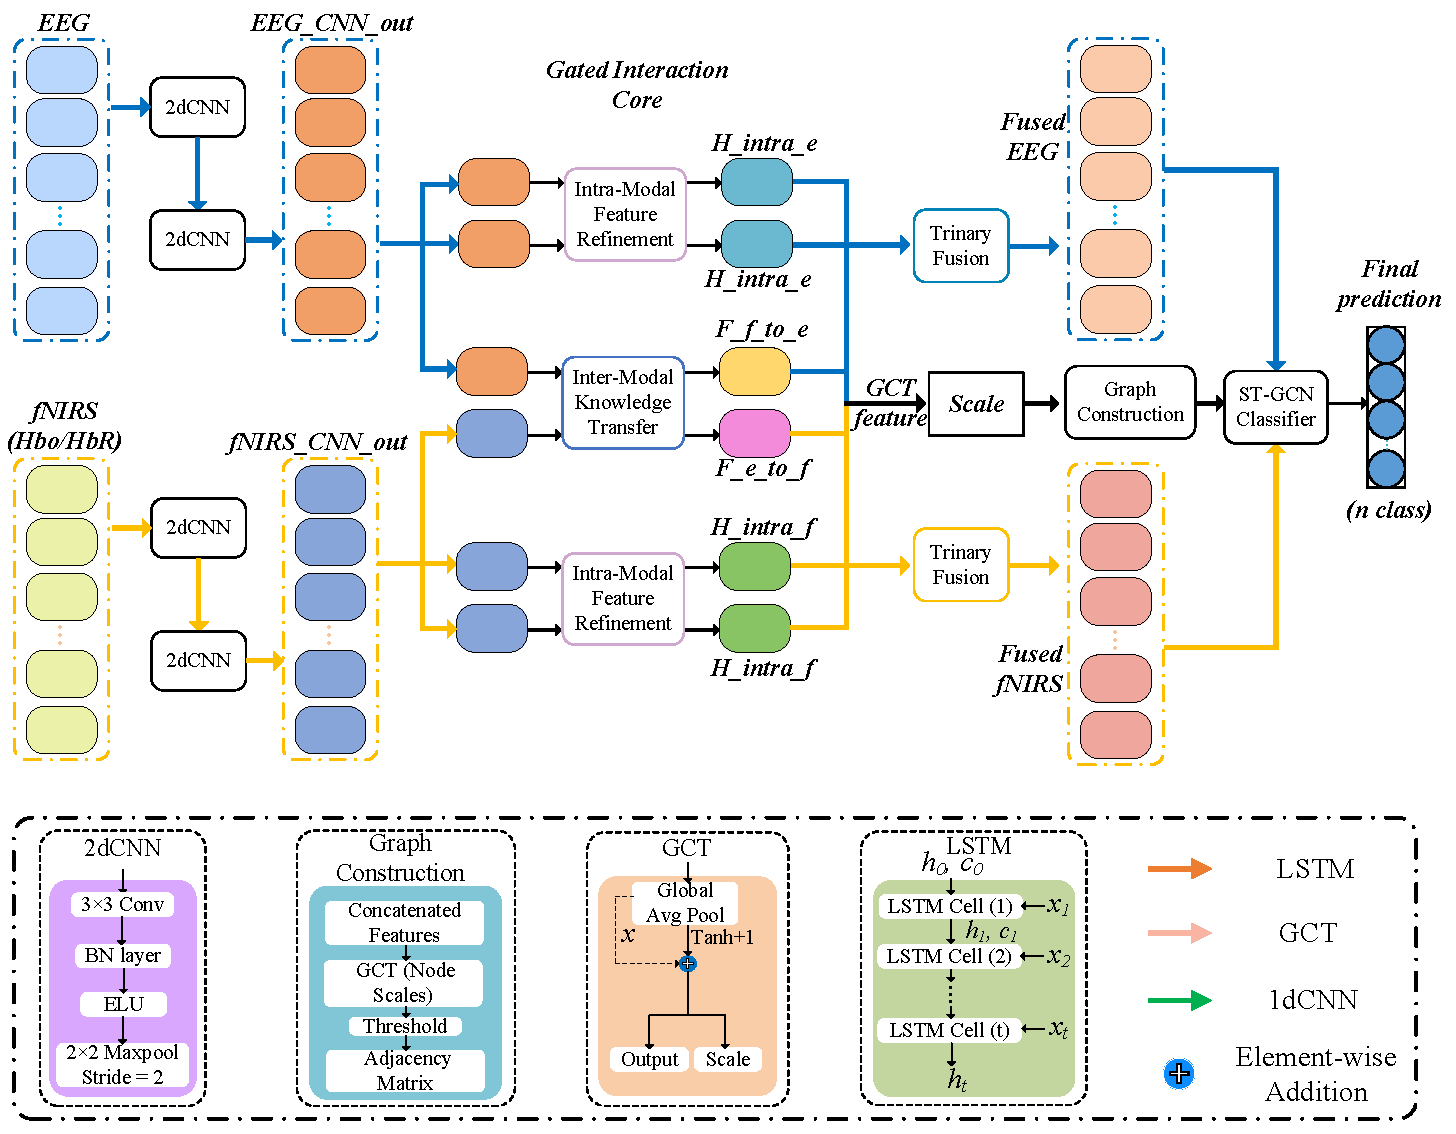
\includegraphics[width=0.75\textwidth]{figures/example-figure.pdf}
    \caption{示例图片}
    \label{fig:example}
\end{figure}

\section{本章小结}
这里填写本章小结。

    \chapter{实验与结果分析}
\label{chapter:experiment}

\section{实验设置}
这里填写实验设置。

\section{结果分析}
表~\ref{tab:example} 是示例表格，学校要的是三线表。

\begin{table}[H]
    \centering
    \caption{示例表格}
    \label{tab:example}
    \begin{tabular}{ccc}
        \toprule
        方法 & 指标一 & 指标二 \\
        \midrule
        方法 A & 0.90 & 0.85 \\
        方法 B & 0.92 & 0.88 \\
        \bottomrule
    \end{tabular}
\end{table}

更复杂的表可以参考表~\ref{tab:comparative_performance}，这里用了 我自己的结果，请修改即可。

\begin{table}[htbp]
	\centering
	\caption{总体性能对比 (mean $\pm$ std)}
	\label{tab:comparative_performance}
	\small
	\resizebox{\textwidth}{!}{
		\begin{tabular}{l ccc ccc ccc}
			\toprule
			\multirow{2}{*}{\textbf{方法}} &
			\multicolumn{3}{c}{\textbf{MI 任务}} &
			\multicolumn{3}{c}{\textbf{MA 任务}} &
			\multicolumn{3}{c}{\textbf{WG 任务}} \\
			\cmidrule(lr){2-4} \cmidrule(lr){5-7} \cmidrule(lr){8-10}
			& Acc. (\%) & F1 (\%) & Sig. & Acc. (\%) & F1 (\%) & Sig. & Acc. (\%) & F1 (\%) & Sig. \\
			\midrule
			EFNet (2024)     & \textbf{80.5 $\pm$ 6.6} & \textbf{76.9 $\pm$ 8.0} & – & 68.6 $\pm$ 7.6 & 57.6 $\pm$ 8.7 & $^{***}$ & 80.1 $\pm$ 6.6 & 74.8 $\pm$ 8.0 & $^{*}$ \\
			ECAfusion (2025)  & 67.9 $\pm$ 8.7 & 55.9 $\pm$ 9.2 & $^{**}$ & 64.6 $\pm$ 4.8 & 52.2 $\pm$ 5.0 & $^{***}$ & 71.4 $\pm$ 7.8 & 64.5 $\pm$ 9.4 & $^{**}$ \\
			STANet (2025)    & 73.9 $\pm$ 6.1 & 63.4 $\pm$ 11.3 & $^{*}$ & 71.5 $\pm$ 9.0 & 63.1 $\pm$ 11.4 & $^{**}$ & 73.9 $\pm$ 6.1 & 63.4 $\pm$ 11.3 & $^{*}$ \\
			M2NN (2022)    & 67.4 $\pm$ 7.2 & 52.7 $\pm$ 6.0 & $^{**}$ & 66.8 $\pm$ 7.4 & 53.0 $\pm$ 6.3 & $^{**}$ & 74.6 $\pm$ 6.5 & 68.9 $\pm$ 7.5 & $^{*}$ \\
			ST2A (2025)   & 72.8 $\pm$ 7.8 & 62.0 $\pm$ 9.7 & $^{**}$ & 72.8 $\pm$ 7.8 & 62.0 $\pm$ 9.7 & $^{**}$ & 77.5 $\pm$ 8.8 & 74.1 $\pm$ 8.8 & – \\
			\textbf{DyGFN (本文)}               & \textbf{80.8 $\pm$ 6.9} & 75.3 $\pm$ 7.3 & \textbf{–} & \textbf{82.1 $\pm$ 6.9} & \textbf{76.6 $\pm$ 6.7} & \textbf{–} & \textbf{80.8 $\pm$ 5.9} & \textbf{75.7 $\pm$ 7.3} & \textbf{–} \\
			\bottomrule
		\end{tabular}
	}
\end{table}

\section{本章小结}
这里填写本章小结。


    \renewcommand{\backref}{}
    \renewcommand{\backrefalt}[4]{}
    \reference{mainref}

    \begin{appendix}
这里填写附录内容。如无附录，可在 main.tex 中注释掉本文件的 include 行。
\end{appendix}

    \begin{achievement}
这里填写攻读学位期间的学术成果。
一般写论文就行了，但是记得和前文的参考文献保存一致
\end{achievement}

    \begin{thanks}
这里填写致谢内容。
\end{thanks}

\end{document}
